% !TEX root =  ./main.tex

\section{Running Example: a Toy Vending Machine}\label{sec:student}

To illustrate some basic concepts of RSs and, in the next section, of the proposed \GROOVE encoding, we model a system composed of a student and a vending machine as a toy example.
The vending machine accepts two different kinds of coins and can dispense either a cappuccino or an expresso when a coffee coin is inserted or a tea if a tea coin is inserted. A cappuccino is dispensed if some milk is available, otherwise expresso is produced.
Assuming the powder for preparing coffee and tea are always present, the corresponding process can be written as follows:
\[
\begin{array}{lll}
\mathsf{VM} & \triangleq & (\{\ccoin,\cpowder\},\{\nomilk\},\{\cappuccino\})\\
& | & (\{\ccoin,\cpowder,\nomilk\},\varnothing,\{\espresso\})\\
& | & (\{\tcoin,\tpowder\},\varnothing,\{\tea\})\\
& | & (\{\cpowder\},\varnothing,\{\cpowder\})\\
& | & (\{\tpowder\},\varnothing,\{\tpowder\})\\
\end{array}
\]

A refill context process can, nondeterministically, refill the machine with milk.
\[
\begin{array}{lll}
\mathsf{Refill} & \triangleq & \{\nomilk\}.\mathsf{Refill}
+ \varnothing.\mathsf{Refill}
\end{array}
\]

The student process is very simple: she takes cappuccino in the morning and tea in the afternoon, otherwise she gets angry.
\[
\begin{array}{rll}
\mathsf{Student} & \triangleq & (\{\am\},\varnothing,\{\ccoin\}).\mathsf{GetCappuccino}\\
& + & (\varnothing,\{\am\},\{\tcoin\}).\mathsf{GetTea}\\
& + & \{\idle\}.\mathsf{Student}\\
\mathsf{GetCappuccino} & \triangleq & (\{\cappuccino\},\varnothing,\varnothing).\mathsf{Student}\\
& + & (\{\espresso\},\varnothing,\{\anger\}).\mathsf{Student}\\
\mathsf{GetTea} & \triangleq & (\{\tea\},\varnothing,\varnothing).\mathsf{Student}\\
& + & (\varnothing,\{\tea\},\{\anger\}).\mathsf{Student}\\
\end{array}
\]
If the student is angry, she will bang the machine:
\[
\begin{array}{lll}
\mathsf{Anger} & \triangleq & (\{\anger\},\varnothing,\{\bang\})
\end{array}
\]
Finally, two more reactions model the passage of time (morning vs afternoon) while the student is idle (i.e., not in the process of getting beverages).
\[
\begin{array}{lll}
\mathsf{Day} & \triangleq & (\{\idle\},\{\am\},\{\am\})\\
& | & (\{\am\},\{\idle\},\{\am\})
\end{array}
\]

We assume that, initially, both entitities $\cpowder$ and $\tpowder$ are present.
So the system is coded as:
%the guarded RS process
\[
[\,\mathsf{Refill}
| \mathsf{Student}
| \{\cpowder,\tpowder\} 
| \mathsf{VM}
| \mathsf{Anger}
| \mathsf{Day}\,] .
\]

The complete encoding of the above RS in \BioResolve syntax is reported in \Cref{fig:bioresolve:toy} in the appendix.
Using the \BioResolve directive \verb=main_do(digraph)=, we can automatically generate the underlying LTS as in \Cref{fig:toylts}: the initial state is in light blue, while there is also a ``bad'' state in which the student is banging the machine, shown in light coral.
Note that, as \am is initially not present, it means that the initial time is in the afternoon.
To improve readability, the nodes of the LTS are labelled by the list of currently active context processes and present entities, and the arcs are labelled by the list of entities provided by the context (see \Cref{rem:shortlts}).\todo{Shorten}
%, i.e., the components in $D\cup C$ extracted from the full label $\obs{\obs{D}{R',I',C}}{R,I,P}$.
% The label $0$ stands for the empty set.
%As a general strategy for \BioResolve, we use a special entity named $\Forbidden$ to mark unwanted states: here the entity is produced thanks to the auxiliary reaction $(\{\anger\},\varnothing,\{\Forbidden\})$.

\begin{figure}
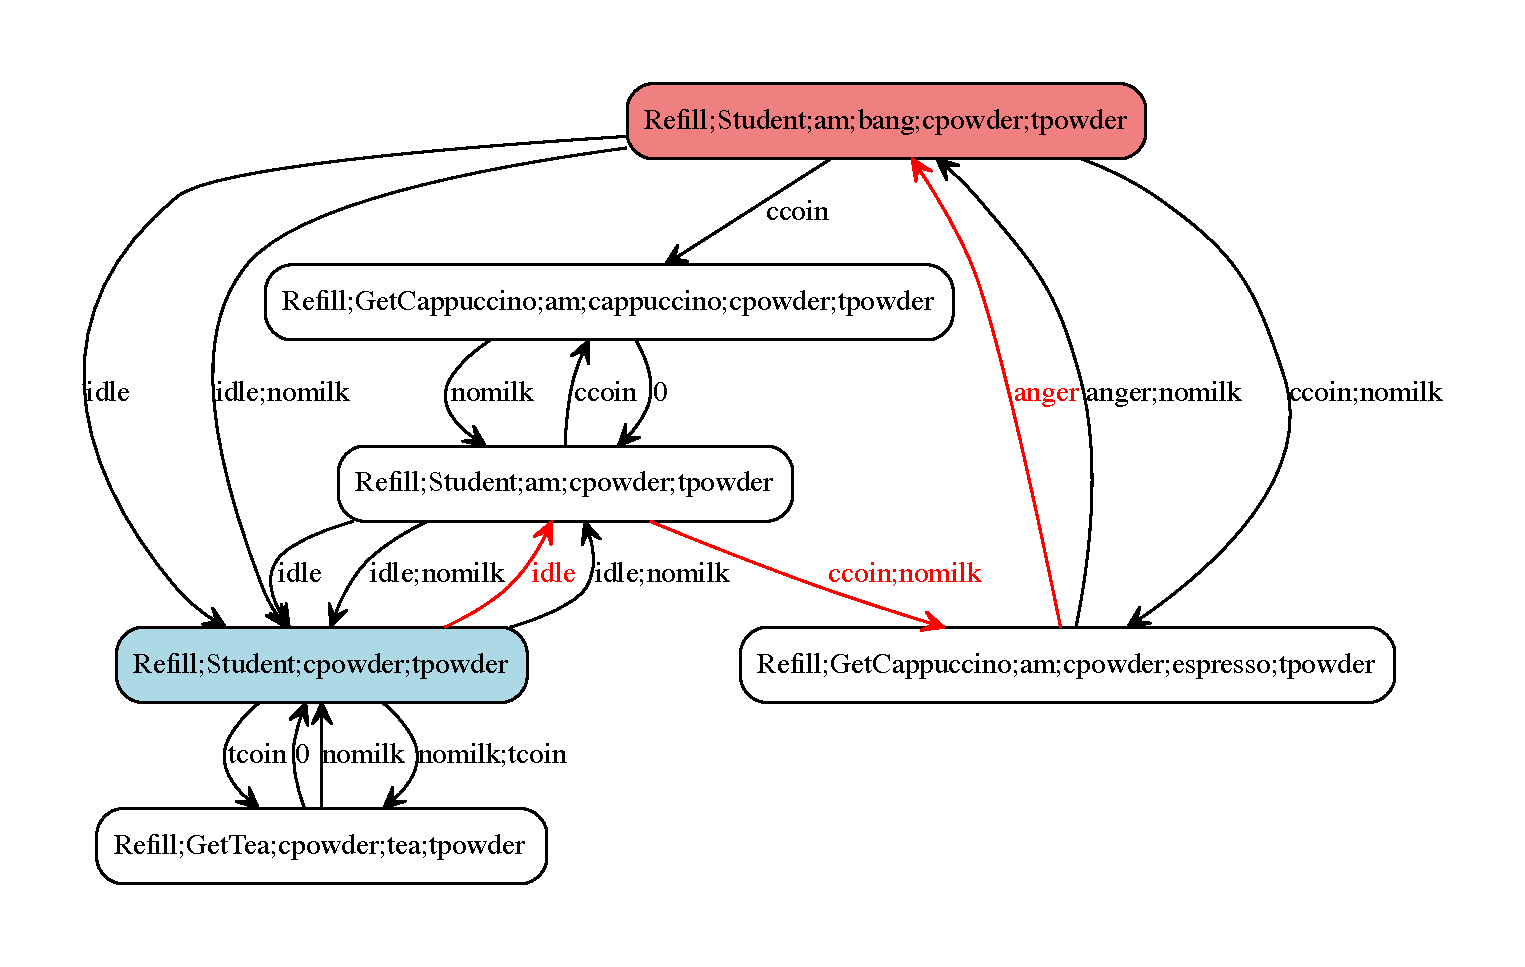
\includegraphics[scale=.3]{./figs/toylts-traced}
\caption{LTS of the toy example. For brevity we use the notation introduced in \Cref{rem:shortlts}, where node labels only account for the list of (semicolons separated) current contexts and entities and transition labels carry the entities provided by the context.\label{fig:toylts}}
\end{figure}

In this particular example, we wish to analyze why \bang is produced, i.e., what are its causes. By manual inspection we can recover a trace starting from the initial state and leading to the ``bad'' state, e.g., $\xrightarrow{\idle}\xrightarrow{\ccoin;\nomilk}\xrightarrow{\anger}$ (highlighted in red in \Cref{fig:toylts}). 
\todo{RB: modified the figure of the LTS to highlight the error trace}
From this trace, using the dynamic slicing process described in~\cite{DBLP:journals/nc/BrodoBF24}, we can reconstruct that the production of \bang was due to the prior production of $\anger$, which in turn was caused by the student getting espresso instead of cappuccino, which is because there was $\nomilk$ when a $\ccoin$ was inserted at $\am$.
